\documentclass[12pt, letterpaper]{article}
\usepackage{graphicx} % Required for inserting images
\usepackage{hyperref}
\usepackage{listings}
\usepackage{amssymb}
\usepackage{amsmath}
\usepackage[english]{babel}
\usepackage{nicefrac, xfrac}
\usepackage{mathtools}
\usepackage[table,xcdraw]{xcolor}
\definecolor{light-gray}{gray}{0.95}
\definecolor{sap}{RGB}{130, 36, 51}
\definecolor{lg}{RGB}{102, 161, 95}
\usepackage[paper=a4paper,left=20mm,right=20mm,bottom=25mm,top=25mm]{geometry}
\newcommand{\code}[1]{\colorbox{light-gray}{\texttt{#1}}}
\newcommand{\shelll}[1]{\colorbox{black}{\textcolor{white}{\texttt{#1}}}}
\newcommand{\shell}[1]{\colorbox{black}{\textcolor{white}{\texttt{casufrost@debian:$\sim$\$ #1}}}}
\newcommand{\codee}[1]{\colorbox{white}{\texttt{#1}}}
\newcommand{\acc}{\\\hphantom{}\\}
\newcommand{\dete}{{\rightarrow}}
\newcommand{\fdot}{{\(\bullet\) }}
\newcommand{\spaz}{{\hphantom{spazio} }}
\newcommand{\boxedMath}[1]{\begin{tabular}{|c|}\hline \texttt{#1} \\ \hline\end{tabular} :}

%sta roba serve per il codice C
\definecolor{mGreen}{rgb}{0,0.6,0}
\definecolor{mGray}{rgb}{0.5,0.5,0.5}
\definecolor{mPurple}{rgb}{0.58,0,0.82}
\definecolor{backgroundColour}{rgb}{0.95,0.95,0.92}

\lstdefinestyle{CStyle}{
    backgroundcolor=\color{backgroundColour},   
    commentstyle=\color{mGreen},
    keywordstyle=\color{magenta},
    numberstyle=\tiny\color{mGray},
    stringstyle=\color{mPurple},
    basicstyle=\footnotesize,
    breakatwhitespace=false,         
    breaklines=true,                 
    captionpos=b,                    
    keepspaces=true,                 
    numbers=left,                    
    numbersep=5pt,                  
    showspaces=false,                
    showstringspaces=false,
    showtabs=false,                  
    tabsize=2,
    language=C
}
%fine roba che serve per il codice C

\title{Sistemi Operativi 2}
\author{Marco Casu}
\date{\vspace{-5ex}}
\begin{document}



\maketitle
\begin{figure}[h]
    \centering{
    
\includegraphics[width=1\textwidth ]{images/cop.jpg}
    }
\end{figure}
\newpage 
\tableofcontents
\newpage
\section{Introduzione}
\subsection{Breve Panoramica su Unix}
Moltissimi sistemi operativi moderni, come \textit{MacOs}, \textit{Linux}, e molti altri, sono basati 
su \textbf{\textit{Unix}}, un sistema operativo il cui sviluppo cominciò nel lontano 1965. Inizialmente implmenetato 
totalmente in assembly, e limitato esclusivamente ad un tipo di architettura, si decise di costruire dei linguaggi 
di programmazione di più alto livello per garantire la portabilità, le versioni di Unix nei linguaggi \textit{B} e 
\textit{C} permisero di portare Unix su diverse CPU.\acc 
Venne distribuito con codice sorgente a centri di ricerca ed università, si diffuse rapidamente e nacquero diverse 
versioni. Le caratteristiche principali di un OS basato su Unix sono le seguenti: \begin{itemize}
    \item Supporta più utenti e la multiprogrammazione 
    \item Il file system ha un organizzazione gerarchica 
    \item Ha un kernel rappresentante il cuore del sistema 
    \item Si interagisce col kernel tramiite le chiamate di sistema
    \item Ha una \textit{shell} (si vedrà in seguito)
    \item È modulare e fornisce ambienti di programmazione
\end{itemize}
È composto da una serie di programmi limitati che eseguono molto bene un compito specifico, presentano un output 
minimale, sono detti "silenziosi", e lavori più complessi possono essere svolti componendo ed articolando diversi programmi 
semplici. I programmi solitamente manipolano file di testo (interpretabili dall'uomo secondo la codifica ASCII) e non file 
binari. Qualsiasi risorsa può essere vista come file o come processo.
\subsection{La Shell}
La \textbf{Shell} non è altro che un programma che esegue dei comandi, che possono essere scritti sul 
terminale, esistono vari tipi di shell, come quella denominata \textit{bash}. La bash scrive il cosiddetto 
\textit{prompt}, ossia una dicitura che indica che il terminale è in attesa di ricevere comandi, molto spesso è 
costituito dal nome dell'utente, il nome del computer, ed il percorso della directory nella quale è aperto il 
terminale.\acc
\shelll{nomeutente@nomemacchina:$\sim$\$} \textit{in attesa di ricevere comandi}
\acc 
Ogni \textbf{comando} seguirà il seguente template : Prima il nome del comando, poi le varie opzioni, e poi gli argomenti 
del comando, ci deve essere almeno un argomento obbligatorio, e zero o più argomenti opzionali, gli argomenti vanno 
separati da un carattere se indicato. \textit{Esempio} :\acc 
\shell{ps -p \$\$ -ocmd -h}
\acc 
Uno dei comandi fondamentali è \code{man}, e sta per \textit{manuale}, è un comando fondamentale che fornisce 
le informazioni più autorevoli possibile riguardo un comando, basta chiamarlo, dando come argomento appunto, il 
nome di un comando, e fornirà una lista dettagliata di tutte le opzioni ad esso correlato.\acc 
\shell{man ps} produce il seguente output : \begin{center}
    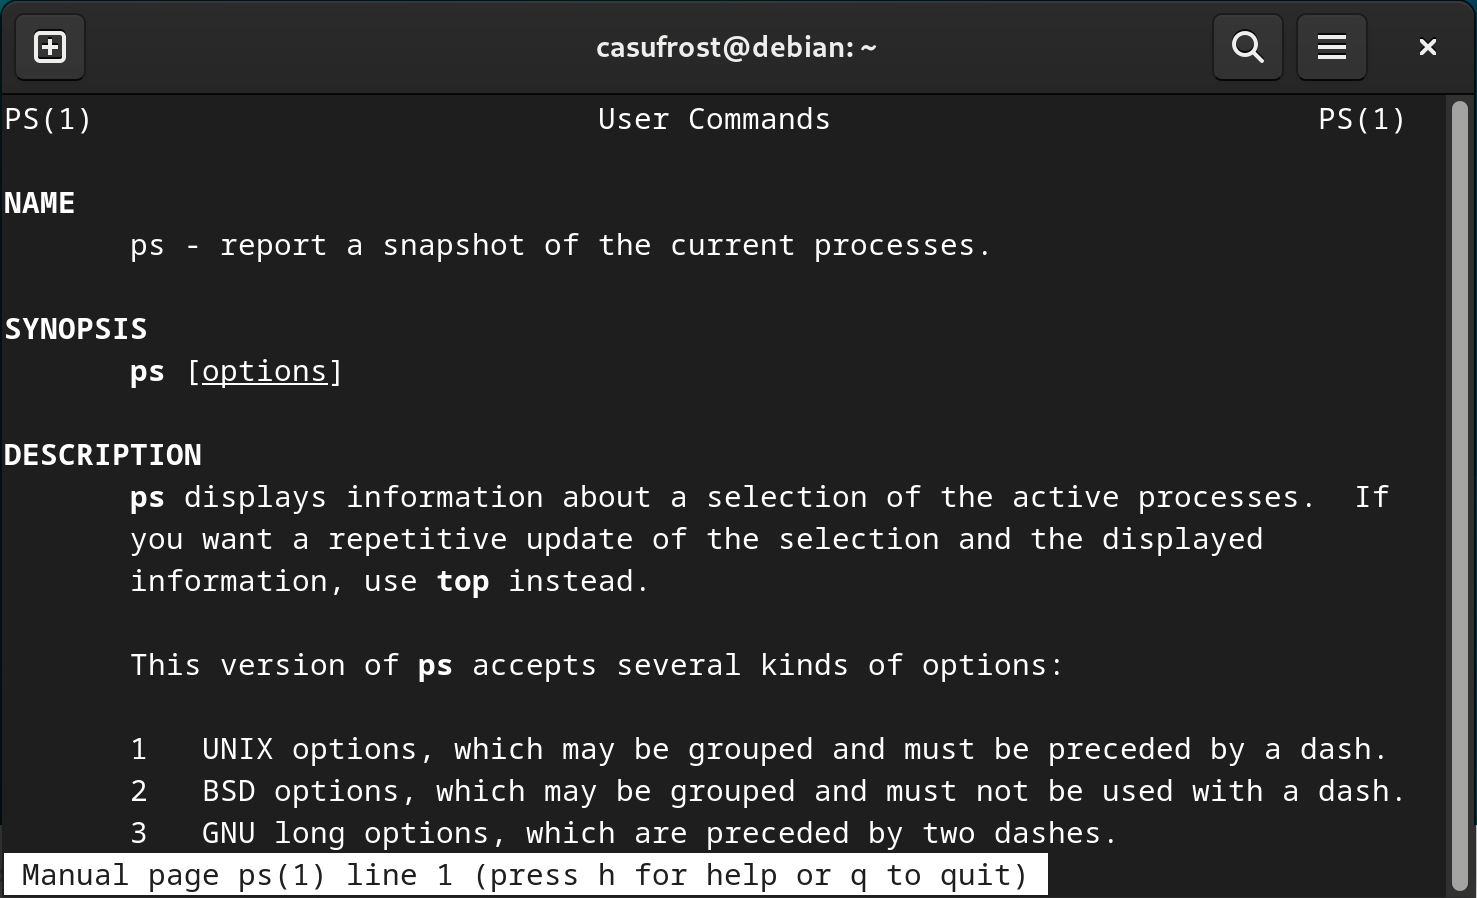
\includegraphics[width=0.7\textwidth ]{images/manPs.png}
\end{center}
Consultando il manuale è possibile capire come utilizzare i comandi fondamentali : 
\begin{itemize}
    \item \shelll{ps} - Mostra le informazioni dei processi attualmente in esecuzione.
    \item \shelll{ls} - Mostra una lista delle risorse contenute in una directory.
    \item \shelll{cp} - Copia file e directory.
\end{itemize}
Analizziamo il comando di esempio scritto in precedenza, ossia: \acc\shell{ps -p \$\$ -ocmd -h} tale comando 
mostra i processi attualmente in esecuzione, l'opzione serve a selezionare il processo in base al suo 
PID, e prede come parametro \code{\$\$}, ossia il codice identificativo del processo bash. \acc Il comando mostra 
varie informazioni, come il PID del processo ed il nome, L'opzione \code{-o} serve a selezionare solo uno dei 
parametri del processo, in questo caso prende come argomento \code{cmd} e seleziona quindi solo quel campo, ossia 
il nome. Si noti come in questo caso non è necessario lasciare uno spazio fra l'opzione e l'argomento. L'ultima opzione, 
ossia \code{-h}, serve a rimuovere il nome dei campi visualizzati, ci si aspetta quindi che tale comando in output 
restituirà esclusivamente il nome del processo bash : \acc 
\shell{ps -p \$\$ -ocmd -h}\\
\shelll{bash}\acc 
Un altro esempio : \acc 
\shell{ps -p \$\$}\\
\shelll{\space\space PID\space\space TTY\space\space\space\space\space\space TIME\space\space\space CMD\space}\\
\shelll{\space 3134\space pts/0\space\space\space 00:00:00\space bash}\acc 
Durante la configurazione di un sistema Unix è necessario specificare almeno un utente. Differenti utenti hanno 
differenti privilegi, l'utente \textbf{root}, o \textbf{superutente}, è predefinito in ogni sistema 
e possiede tutti i privilegi, è detto \textit{amministratore di sistema}.\acc 
Tale utente però, non può effettivamente eseguire un login ed entrare nel sistema, se necessario eseguire un 
operazione privilegiata, gli altri utenti possono acquisire temporaneamente i diritti di amministratore tramite 
il comando \shelll{sudo}, acronimo di \textit{super user do}.\acc 
Gli utenti appartengono a dei \textit{gruppi} che definiscono diversi privilegi, coloro che possono richiedere 
temporaneamente i diritti di amministratore appartengono al gruppo dei \textit{sudoers}, è possible mostrare 
a quali gruppi appartiene un utente tramite il comando \shelll{groups}.\acc 
\shelll{sudo} è un comando che prende come input un altro comando da eseguire in modalità root, esiste anche un altro 
comando chiamato \shelll{su}, e sta per \textit{substitute user}, e serve per cambiare utente, e diventare 
possibilmente amministratore, risulta comunque meno sicuro del comando \shelll{sudo}, in quanto quest'ultimo 
permette solo di eseguire un operazione in maniera privilegiata, senza rimanere nella condizione di root.
\section{Il File System}
La gestione dei file in un sistema Unix non è delegata al kernel, essi non risiedono infatti in quest'ultimo, e più file system 
possono coesistere nello stesso sistema : diversi dischi (o altre unità di archiviazione) possono gestire i file in maniera
 diversa. Tutti i file convivono sotto la stessa cartella radice, detta \textit{root}, in maniera totalmente trasparente.\acc 
 Il file system gestisce la memoria secondaria ed è organizzato in maniera \textbf{gerarchica}, vi è una \textit{directory}
  (cartella) principale che si trova alla radice dell'albero, che si dirama in più directory fino ad arrivare alle foglie, 
  ovvero i file (che non possono ospitare altri file), è una struttura ricorsiva. Ci sono due tipi di file in Unix : \begin{itemize}
    \item \textbf{file non regolari} - Quei file che danno un \textit{accesso astratto} a periferiche e dispositivi, come già
    accennato, in Unix tutto può essere visto come un file o come un processo, de facto anche lo stesso mouse viene modellato come 
    un file, e sarà appunto un file di questo tipo.
    \item \textbf{file regolari} - Tutti i restanti file ordinari, come un file di testo o l'eseguibile di un programma.
  \end{itemize}
La directory root è indicata dal simbolo \shelll{/}, tutto è contenuto in tale cartella, anche una chiavetta USB che viene 
inserita nella macchina, i drive riceveranno una cartella sotto la root. Il file system impone alcune restrizioni sui nomi dei file : \begin{itemize}
    \item Non è possibile creare due file con lo stesso nome nella stessa directory.
    \item Non è possibile creare due directory con lo stesso nome nella stessa directory.
    \item Non è possibile creare una directory ed un file con lo stesso nome nella stessa directory.
\end{itemize}
\subsection{Operazioni sulle Directory}
Ogni singolo file del file system è raggiungibile mediante un cammino detto \textit{path}, una sequenza di nomi di directory 
separate dal carattere \shelll{/} che indicano la locazione del file, tale path può essere assoluto o relativo. In ogni sistema 
Unix, la directory \textit{home} dell'utente può anche essere indicata con il carattere \shelll{\(\sim\)}, infatti, i seguenti 
due path sono equivalenti : \acc 
\shelll{\(\sim\)/Immagini(faces)}\\
\shelll{home/Immagini(faces)}\acc
Nella shell, viene sempre visualizzata la directory corrente nella quale ci si trova, che di default è home appena si apre il 
terminale, cambiando la directory cambierà anche la dicitura che indica la current directory sul prompt.
\subsubsection{Comandi di Base}
Il comando \shelll{cd}, che sta per \textit{change directory}, serve a cambiare la directory corrente, e richiede come 
argomento un path, che può essere assoluto o relativo, se relativo, si riferirà alle directory contenute nella current directory, altrimenti 
si può dare il cosiddetto path assoluto, specificando la posizione a partire dalla root.\acc 
\shell{cd Immagini}\spaz per spostarsi nella cartella immagini\\
\shelll{casufrost@debian:$\sim$/Immagini\$}\acc 
Se non si passa alcun argomento, il comando sposta l'utente nella home. È possibile riferirsi alla directory padre 
con \shelll{cd ..} o alla directory corrente con \shelll{cd .}.\acc 
È possibile creare nuove cartelle con il comando \shelll{mkdir}, che sta per \textit{make directory}, prende come argomento 
il path di una cartella, se essa non esiste, verrà creata, è possibile utilizzare l'opzione \code{-p} per creare 
tutto un intero path specificato, creando l'intero cammino in un solo comando.\acc Un path assoluto è valido in qualunque caso, un 
path relativo è ovviamente dipendente dalla current directory, potrebbe quindi risultare non valido. Supponiamo che nel file 
system esista il seguente path : \code{home/animal/dog}, si avrà che : \acc 
\shell{cd dog} Non è valido, funzionerebbe se fossimo in \code{animal}\\
\shell{cd /home/casufrost/animal/dog} assoluto, quindi valido\acc 
Un altro comando estremamente utile è \shelll{ls}, che sta per \textit{list segments}, prende come argomento una directory (se 
omesso considera quella corrente), e mostra tutti i contenuti all'interno di essa, l'opzione \code{-l} mostra ulteriori informazioni 
utili, come i permessi di lettura o scrittura (verrà approfondito in seguito). \acc 
In Unix i file che iniziano con il punto, ad esempio \code{.secret.txt} sono nascosti, è possibile visualizzarli con il 
comando \shelll{ls -a}.\acc 
Esistono altri comandi secondari piuttosto utili : \shelll{tree} mostra l'alberazione della directory, \shelll{touch} crea 
un file vuoto, \shelll{pwd} stampa a schermo la directory corrente.
\subsection{Struttura del File System}
\subsubsection{Mounting e Partizioni}
Il file system può contenere dischi di memoria secondaria, anche dischi in reta, o addirittura una porzione della RAM, tutto 
grazie al meccanismo di \textbf{mounting}, ossia l'operazione di attaccare la radice del file system di un unità secondaria, ad una 
cartella appartenente al file system principale, ossia quello della radice root. \begin{center}
    \includegraphics[width=0.8\textwidth ]{images/mounting.eps}
\end{center}
Una qualsiasi directory dell'albero principale può diventare un \textit{punto di mount} di una qualsiasi altro 
file system, l'unico fatto da considerare è il seguente : Se viene montato un disco su una directory contenete dei file, 
tali file non saranno accessibili finché il mounting verrà rimosso, è quindi opportuno montare i dischi su directory vuote.\acc 
Un disco, può essere anche \textbf{partizionato}, ossia diviso in unità logiche disgiunte che il sistema operativo vedrà come 
 dischi differenti, è solito partizionare il disco in modo da avere un unità per il sistema operativo (che viene montata sulla 
 root) ed un unità per i dati dell'utente (che viene montata sulla home).
 Partizionare il disco risulta comodo ed aumenta il grado di sicurezza nell'organizzazione dei file, se dovesse accadere qualcosa 
 all'unità dell'OS, i dati utente non rimarrebbero corrotti. \acc 
 Linux funziona con diversi tipi di file system, un file system piuttosto utilizzato è quello di tipo \textit{Journal}, esso 
 tiene traccia di tutte le operazioni da eseguire sul disco, in caso di problemi ad esso, consultando il "diario", è possibile 
 avere informazioni riguardo le operazioni eseguite, e le operazioni da eseguire ma non completate, riducendo il danno.\acc 
 Diversi file system differiscono in caratteristiche quali : \begin{itemize}
    \item Dimensione massima delle unità di una partizione 
    \item Dimensione massima di un file
    \item Lunghezza massima per il nome di file o directory
 \end{itemize}
 In unix esistono due importanti file che tengono traccia dei dischi montati, il file \code{/etc/fstab} contiene informazioni 
 sui dischi montati all'avvio della macchina, \code{/etc/mtab} contiene informazioni sui dischi montati dinamicamente dall'utente, è 
 possibile visualizzare il contenuto di questi file (come di un qualsiasi altro file) tramite il comando \shelll{cat}.
 \subsubsection{Inode e Metadati}
 Come vengono gestiti i file all'interno del file system, o meglio, quale struttura dati è impiegata? Esiste una struttura chiama 
 \textbf{inode}, contenente ogni singolo file, identificato da un codice univoco detto \textit{inode number}, fisicamente quindi 
 non vi è un implementazione ad albero/gerarchica.\acc 
 Quando un file viene eliminato, non viene realmente cancellato fisicamente, viene solamente etichettato come "libero" l'inode 
 number ad esso associato, permettendo a nuovi eventuali file di venire associati a quel numero. Il numero totale di entrate 
 nell'inode è elevatissimo ma limitato, esiste quindi un limite al numero di file che possono coesistere nel sistema.\acc 
 Ogni file ha quindi un entrata nell'inode, che ne specifica il codice, ed altri \textit{metadati} utili riguardanti il file, 
 essi sono : \begin{itemize}
    \item Type - il suo tipo, se regolare o non regolare 
    \item User Id - l'Id dell'utente proprietario del file 
    \item Group Id - l'Id del gruppo primario del proprietario 
    \item Mode - permessi di lettura, scrittura ed accesso, riguardanti il proprietario, il gruppo del proprietario e 
    tutti gli altri  utenti
    \item Size - le dimensioni in byte del file 
    \item Timestamps - 3 marcature temporali riguardanti l'istante di cambiamento di un metadato, modifica e lettura del file.
    \item Data pointers - puntatore alla lista di blocchi che compone il file.
 \end{itemize} 
 Le directory contengono informazioni sugli inode number dei file che contengono, permettendo al sistema di seguire i percorsi 
 specificati dall'utente. Tramite il comando \shelll{ls -i},  è possibile visualizzare 
 l'inode number  nel terminale.\subsection{Permessi di Accesso}
 Nei metadati di un file, sono contenute delle informazioni riguardanti l'accesso, appunto del file, da parte dei vari utenti 
 che co-abitano l'ambiente di sistema. \begin{quote}
Supponiamo che il sig. Rossi per non perdere traccia dei suoi accessi ai vari servizi 
 online, si scriva tutte le sue password su un file di testo, che salva sul desktop. Il sig. Verdi, accede al medesimo sistema 
 (ovviamente con un utente differente), esso può visualizzare le password del sig. Rossi?    
\end{quote}
Ogni file contiene dei bit che definiscono i permessi di accesso per i vari utenti, esistono 3 diversi tipi di accesso : \begin{itemize}
    \item \code{r} - \textit{read}, accesso in lettura 
    \item \code{w} - \textit{write}, accesso in scrittura 
    \item \code{x} - \textit{execute}, accesso in esecuzione
\end{itemize}
Quest'ultimo è valido per le directory, una directory con l'accesso \code{x} può essere navigata. Per un file eseguibile non ha 
senso l'accesso \code{x} singolarmente, in quanto è necessario anche che il file venga letto.
Quindi ogni file ha 3 bit, che ne identificano gli accessi, essendo 3 bit, possono anche essere visti come un
numero intero da 0 a 7.\begin{center}
    \begin{tabular}{l|c|c|l|c|}
        \cline{2-5}
        \rowcolor[HTML]{C0C0C0} 
        \cellcolor[HTML]{FFFFFF}{\color[HTML]{FFFFFF} } & 4                                                 & 2                                                 & 1                         & permessi                \\ \hline
        \rowcolor[HTML]{EFEFEF} 
        \multicolumn{1}{|l|}{\cellcolor[HTML]{EFEFEF}0} & -                                                 & -                                                 & -                         & nessun permesso         \\ \hline
        \rowcolor[HTML]{EFEFEF} 
        \multicolumn{1}{|l|}{\cellcolor[HTML]{EFEFEF}1} & -                                                 & -                                                 & \code{x}& solo esecuzione         \\ \hline
        \rowcolor[HTML]{EFEFEF} 
        \multicolumn{1}{|l|}{\cellcolor[HTML]{EFEFEF}2} & -                                                 & \code{w}                        & -                         & solo scrittura          \\ \hline
        \rowcolor[HTML]{EFEFEF} 
        \multicolumn{1}{|l|}{\cellcolor[HTML]{EFEFEF}3} & -                                                 & \cellcolor[HTML]{EFEFEF}\code{w}& \code{x}& scrittura ed esecuzione \\ \hline
        \rowcolor[HTML]{EFEFEF} 
        \multicolumn{1}{|l|}{\cellcolor[HTML]{EFEFEF}4} & \cellcolor[HTML]{EFEFEF}\code{r} & -                                                 & -                         & solo lettura            \\ \hline
        \rowcolor[HTML]{EFEFEF} 
        \multicolumn{1}{|l|}{\cellcolor[HTML]{EFEFEF}5} & \cellcolor[HTML]{EFEFEF}\code{r} & -                                                 & \code{x}& lettura ed esecuzione   \\ \hline
        \rowcolor[HTML]{EFEFEF} 
        \multicolumn{1}{|l|}{\cellcolor[HTML]{EFEFEF}6} & \cellcolor[HTML]{EFEFEF}\code{r} & \cellcolor[HTML]{EFEFEF}\code{w}& -                         & lettura e scrittura     \\ \hline
        \rowcolor[HTML]{EFEFEF} 
        \multicolumn{1}{|l|}{\cellcolor[HTML]{EFEFEF}7} & \cellcolor[HTML]{EFEFEF}\code{r} & \cellcolor[HTML]{EFEFEF}\code{w}& \code{x}& tutti i permessi        \\ \hline
        \end{tabular}
\end{center}
Il fatto è che non esiste una sola tripla di bit, ma ne esistono ben 3, la prima identifica i permessi per l'utente proprietario 
del file in questione, la seconda identifica i permessi per gli utenti che appartengono al gruppo primario del proprietario del file, 
la terza identifica i permessi per tutti gli altri utenti. Ad esempio, se il file \code{frost.txt} ha i permessi 
\code{rwx,rwx,r--} o \code{774} può essere letto, scritto ed eseguito dal proprietario e dai membri del suo gruppo primario, 
mentra può essere esclusivamente letto da tutti gli altri utenti.
\acc
Esistono inoltre 3 ulteriori bit nei metadati di ogni file che consentono ulteriori permessi : \begin{itemize}
    \item \textbf{sticky bit} - Serve a proteggere le directory ed il loro contenuto dagli utenti non proprietari, un file in una 
    directory può essere acceduto da chi ha i permessi della directory ma non del file, con lo sticky bit, sarà necessario 
    essere proprietario del file in questione.
    \item \textbf{setuid bit} - Utilizzato esclusivamente per i file eseguibili, permette a coloro che eseguono il 
    file in questione di ottenere momentaneamente gli stessi permessi del proprietario del file, ad esempio il comando 
    \shelll{passwd} sfrutta tale bit, e permette ad un utente di modificare la propria password anche se il proprietario 
    del file è l'utente root.
    \item \textbf{setgid bit} - Analogo al precedente, ma riguardante il gruppo.
\end{itemize}
È possibile modificare i permessi di accesso ad un file tramite il comando \shelll{chmod}, specificando prima la tripla di ottali 
che identificherà i nuovi permessi, e poi il file in questione, è possibile anche cambiare il proprietario ed il gruppo di un 
file tramite \shelll{chown} e \shelll{chgrp}, se abbinati con l'opzine \shelll{-r}, tutti i sottoalberi dell'argomento 
riceveranno lo stesso trattamento.\acc Un importante valore di un sistema operativo Unix è la  \textit{user mask}, ossia 
una parola di bit che identifica i permessi di default che vengono assegnati ad un file nel momento della sua creazione.
La user mask è composta da quattro terne di 3 bit (rappresentanti i permessi ed i permessi speciali), e può essere modificata 
con il comando \shelll{umask} inserendo come parametro la nuova maschera.\acc 
I permessi di default di ogni file sono calcolati nel seguente modo : \begin{center}
    \code{111 111 111 111 AND NOT(\{user mask\})}
\end{center}
Ad esempio (escludendo i bit speciali) per impostare i diritti di default a 664, bisognerà performare il seguente comando : \begin{center}
    \shelll{umask 113}  \code{111 111 111 AND NOT(001 001 011) = 111 111 111 AND 110 110 100 = 110 110 100 = 664}
\end{center}
Altri comandi fondamentali per manipolare i file sono\begin{itemize} \item \shelll{cp} : Permette di copiare un file in una destinazione specificata
    \item \shelll{mv} : Permette di spostare un file in una destinazione specificata \item\shelll{rm} : Elimina il file specificato\acc 
\end{itemize}
Abbiamo poi visto che è possibile creare dei \textit{link o collegamenti} fra file, un \textit{soft link}, sarà un file che conterrà 
il puntatore ad un altro file, un \textit{hard link}, sarà invece un altro file, ma con il riferimento allo stesso inode number,
saranno quindi due file distinti, senza che però il disco sia occupato due volte.\acc 
È possibile creare dei link con il comando \shelll{ln}, l'eliminazione del file originale nega l'accesso a tutti 
i soft link ad esso collegati, per eliminare un file di cui invece esistono più hard link, bisogna eliminarli tutti.\acc 
Passiamo ora ad un comando particolare, ossia \shelll{dd}, tale comando è presente anche in delle primordiali versioni di Unix, e 
serve a copiare i file in maniera più sofisticata, opzionalmente effettuando conversioni, i suoi parametri assumono la 
sintassi \shelll{variabile=valore}, differentemente dal simbolo \shelll{-} utilizzato per gli altri comandi.\acc 
Può leggere e copiare i file \textit{byte per byte}, specificando il numero preciso di blocchi da copiare, la dimensione 
di tali blocchi, e 
dove scriverli all'interno del file di destinazione, a tal scopo ci sono le opzioni \code{count,bs,skip,of,if,seek}, ad esempio : \begin{itemize}
    \item \shelll{skip=x} - Del file da copiare, verranno ignorati i primi $x$ blocchi.
    \item \shelll{seek=x} - Nel file di destinazione, il contenuto verrà copiato a partire dal $x$-esimo blocco. 
\end{itemize}
\section{I Processi in Unix}
Abbiamo già accennato al fatto che in Unix ogni entità può essere vista come un file, le due componenti fondamentali di un 
sistema di questo tipo però, non sono esclusivamente i file, ma anche i \textit{processi}. Un processo 
rappresenta l'istanza di un programma/file eseguibile che viene avviato e caricato sulla memoria
principale, una volta avviato, l'OS si occuperà di tale processo, come i file, ogni processo è identificato da un numero 
intero univoco.\acc 
Per avviare un programma, e renderlo un processo, bisogna digitare sulla shell il codice del programma da eseguire, quando 
vengono richiamati i comandi \shelll{dd,ls,cat} e \shelll{cp}, vengono eseguiti dei nuovi processi, differentemente, i 
programmi \shelll{echo} e \shelll{cd}, che sono comandi interni, fanno parte del processo shell.\acc 
Uno stesso programma può essere istanziato più volte, dando vita a più processi copia di uno stesso programma che girano sulla 
macchina.
\subsection{Canali di Input/Output}
Ogni processo di Unix ha accesso a 3 canali/file di default, utili per il flusso di dati in input ed output, questi sono : \begin{itemize}
    \item \code{stdin} (\textit{standard input}) : Per il flusso di dati in input, ha il codice descrittore uguale a 0, e di default è impostata 
    la tastiera.
    \item \code{stdout} (\textit{standard output}) : Per il flusso di dati in output, ha il codice descrittore uguale a 1, e di default
    è impostato lo schermo.
    \item \code{stderr} (\textit{standard error}) : Secondo canale di output utile per eventuali errori e diagnostica, 
    ha il codice descrittore uguale a 1, e di default è impostato lo schermo.
\end{itemize}
I 3 canali possono essere "ridirezionati" dall'utente in maniera indipendente, ad esempio, è possibile cambiare il flusso di dati 
in output, facendo si che \code{stdout} venga impostato su un file, tutti i dati in output di un programma potranno quindi 
essere scritti su un file specificato, vale lo stesso principio per la lettura con \code{stdin}.\acc A tale scopo, quando 
si avviano i programmi dalla shell, bisogna utilizzare i simboli \code{<} e \code{>} per ridirezionare rispettivamente 
l'input e l'output, ad esempio : \acc 
\shell{ls > dirlist} : scriverà il risultato del comando sul file \code{dirlist}.\acc 
Il precedente citato \textit{descrittore di un file} è un identificatore univoco per ogni file, similmente all'inode, ma di 
più alto livello.
\subsection{Struttura di un Processo}
Ogni processo è identificato dal sistema con un codice 
univoco, un numero intero detto \textit{PID}. Oltre ciò, 
ogni processo ha un \textit{Process Control Block} (PCB), e 
6 aree di memoria dedicata.\acc 
Il PID 0 è assegnato ad un processo chiamato 
\code{init}, è il primo processo avviato dalla macchina e 
si occupa di avviare tutti gli altri processi. Quando un 
processo termina, il suo PID viene liberato, alcuni sistemi per 
ragioni di sicurezza assegnano i PID in maniera casuale.
Il PCB è una struttura dati contenente dei valori che forniscono 
informazioni su ogni processo, contiene: \begin{itemize}
    \item \textit{PID} - Il suo codice identificativo 
    \item \textit{PPID} - Il PID del suo processo padre
    \item \textit{Real UID} - Id dell'utente proprietario 
    \item \textit{Real GID} - Id del gruppo dell'utente proprietario 
    \item \textit{Effective UID} - Id effettivo dell'utente assunto
    \item \textit{Effective GID} - Id effettivo del gruppo dell'utente assunto
    \item \textit{Saved UID} - UID avuto prima dell'esecuzione del SetUID
    \item \textit{Saved GID} - Analogo al precedente ma per il gruppo 
    \item \textit{Current Working Directory} - La directory dalla quale è stato avviato il processo
\end{itemize}
Il \textit{Saved UID} permette ad un processo in esecuzione come root, di eseguire delle operazioni in veste di utente 
non privilegiato, è importante ridurre al minimo (per ragioni di sicurezza) l'utilizzo dei privilegi di root. All'avvio di 
ogni processo, vengono riservate le 6 aree di memoria in seguito : \begin{enumerate}
    \item \textit{Text Segment} - Le istruzioni sequenziali del programma in linguaggio macchina.
    \item \textit{Data Segment} - I dati statici del programma inizializzati caricato, come le variabili globali.
    \item \textit{BSS} - I dati statici del programma non inizializzati, distinto dal Data Segment per motivi di realizzazione
    hardware.
    \item \textit{Heap} - I dati dinamici generati dal processo, ad esempio, la memoria che si riserva con la funzione \code{malloc}.
    \item \textit{Stack} - Pila necessaria per il funzionamento delle chiamate di funzione, con i corrispondenti dati dinamici, come 
    i parametri passati.
    \item \textit{Memory Mapping Segment} - Tutto ciò che riguarda le librerie esterne necessarie al processo.
\end{enumerate}
Per comunicare, più processi potrebbero condividere alcune aree di memoria, come l'heap, oppure se sono caricati due processi 
istanza dello stesso programma, non è necessario avere due distinti text segment, in quanto condividono le stesse istruzioni. Un 
processo in memoria, può trovarsi in uno dei seguenti stati : \begin{itemize}
    \item \textbf{Running} - Il processo è in esecuzione sulla CPU.
    \item \textbf{Runnable} - Il processo è pronto per essere eseguito, ed è in una coda in attesa di essere selezionato dallo
    scheduler.
    \item \textbf{Sleeping} - Il processo non può essere eseguito, in quanto è in atteso di un certo evento, come un segnale di Input 
    da parte dell'utente.
    \item \textbf{Zombie} - Il processo è stato eliminato e le sue aree di memoria liberate, tuttavia il suo PCB è ancora 
    mantenuto, in quanto il processo padre che l'ha generato non ha richiesto che il processo figlio venisse abortito.
    \item \textbf{Stopped} - Non è altro che un particolare caso dello stato \textit{Sleeping}, anche se il processo potrebbe 
    continuare la sua esecuzione, esso è fermo in quanto ha ricevuto un segnale esterno (dall'utente o da un processo) di fermarsi.
    \item \textbf{Traced} - in esecuzione di debug, oppure in generale in attesa di un segnale (altro caso
    particolare di sleep, verrà trattato in seguito).
    \item \textbf{Uninterruptible Sleep} - Un caso di \textit{Sleeping} in cui il processo sta facendo operazioni di I/O molto 
    lunghe su un disco molto lento, facendo si che si trovi in uno stato di attesa appartenentemente interminabile.
\end{itemize}
Un processo, può essere eseguito in \textbf{foreground}, ossia sulla shell dalla quale è stato avviato, prendendone il controllo, 
e solamente una volta che terminerà la sua esecuzione l'utente potrà nuovamente interagire con la shell, oppure in
\textbf{background}, lasciando la shell libera all'utente, e venendo eseguito comunque, a patto che non possa ricevere 
input da tastiera grazie alla shell, riducendone l'interattività. Si può richiedere ad un comando di venire eseguito in 
background con il simbolo \code{\&} :\acc
\shell{ls / -l \&}
\acc
La lista di tutti i processi in esecuzione può essere visualizzata con il comando \shelll{job}, inoltre, è possibile 
spostare un processo da uno stato di background ad uno stato di foreground con il comando \shelll{fg}, oppure
fare l'operazione analoga ma inversa con il comando \shelll{bg}, specificando il PID del processo in questione.
\subsection{Pipelining e Segnali}
L'idea del \textit{pipelining} è quella di creare programmi complessi, concatendando gli output e gli input di piccoli 
programmi più semplici (come appunto è nella filosofia di Unix). Il simbolo \code{|} fra due comandi Unix permette di 
concatenare l'Output del comando alla sua sinistra con l'input del comando alla sua destra, ad esempio \shelll{comando1 | comando2}
farà si che l'input di \shelll{comando2} sarà l'output di \shelll{comando1}. \acc Le informazioni relative ai processi, quali PID, 
nome comando, tempo di esecuzione ed altre possono essere visualizzate con il comando \shelll{ps}, che sta per \textit{processes},
con l'opzione \code{-o} è possibile scegliere quali dati visualizzare. Sono particolarmente utili le opzioni \code{-a} : visualizza 
tutti i processi, e \code{-x} : visualizza i processi che non hanno un terminale.\acc
Il comando \shelll{top} è una versione "interattiva" del comando \shelll{ps}, prende il controllo della shell e funziona in
tempo reale, mostrando i processi che eventualmente vengono creati o terminati.\acc 
Il comando \shelll{kill -[codice] \%PID\%} serve per inviare segnali ai processi, prende in ingresso il codice di uno specifico 
segnale ed il PID di un processo, ad esempio : \acc \shell{kill -9 4562}\acc 
Con il comando \shelll{kill -l} è possibile visualizzare tutti i segnali che possono essere inviati, i più 
comuni sono: \begin{itemize}
    \item \code{SIGSTP} - Per la sospensione di un processo 
    \item \code{SIGCONT} - Per la continuazione di un processo 
    \item \code{SIGKILL} o \code{SIGINT} - Per la terminazione di un processo.
\end{itemize}
Il comando \shelll{nice} serve ad assegnare ad un processo un certo grado di priorità, che lo avvantaggierà nell'essere 
selezionato dallo scheduler, il range della priorità va da -19 a +20.
\section{Il Linguaggio C}
Il linguaggio C è uno dei più antichi linguaggi mai sviluppati, è stato creato dagli autori di Unix negli anni 70 ed è ancora 
in uso. Il C è nato per poter scrivere il kernel di Unix in un linguaggio di più alto livello, in modo da renderlo portatile 
su differenti architetture, è un linguaggio \textit{indipendente} dalla macchina e può essere eseguito su diversi 
sistemi con poche modifiche nel codice (previa eventuale ricompilazione).\acc 
Il \textit{workflow} per la scrittura di un programma in C è la seguente : \begin{enumerate}
    \item Si scrive il programma su un editor di testo.
    \item Si chiama il preprocessore, che si occuperà di "semplificare" il codice.
    \item Si chiama il compilatore, che dal file sorgente genererà le istruzioni in linguaggio macchina. 
    \item Il Linker collegherà l'assemblatore con le eventuali librerie esterne.
\end{enumerate}
I punti (2) e (4) sono spesso gestiti dal compilatore, quindi sarà necessario scrivere il programma, compilarlo per poi 
eseguirlo. Verrà utilizzato il compilatore open-source della GNU, ossia \textit{gcc}.\acc 
Sappiamo che un codice scritto in Java viene compilato in bytecode, per poi venire interpretato dalla \textit{Java Virtual Machine},
 e non direttamente dal processore. La compilazione di un programma C invece, genera un codice del tutto eseguibile, in quanto 
sono istruzioni interpretabili direttamente dal processore, rendendolo quindi più efficente. Necessariamente, un file eseguibile 
scritto in C, deve avere i permessi di esecuzione garantiti.\acc 
Gli strumenti per la scrittura di un programma in C sono il compilatore ed un editor di testo, basterà scrivere il codice per 
poi richiamare dalla shell il compilatore con il comando \shelll{gcc}, la "struttura" di un programma C è fissata, ci deve 
sempre essere una funzione chiamata \code{main()}, ed è la prima funzione che viene chiamata all'avvio del programma quando viene 
caricato in memoria.\acc 
Ovviamente possono essere incluse anche altre funzioni che implementano ulteriori operazioni, è buona regola non scrivere tutto il 
programma in C, ma suddividere il tutto in apposite funzioni, possono essere scritte in un unico file, o anche in più file diversi, 
la compilazione genererà comunque un solo eseguibile.
\subsection{Sintassi}
Una funzione in C ha un intestazione, un tipo di ritorno, dei parametri ed un blocco di codice associato.
\begin{lstlisting}[style=CStyle]
    
    return_type function_name(parameter list)
    {
       blocco di istruzioni
    }
    \end{lstlisting}
I blocchi in C vengono aperti e chiusi dalle parentesi graffe, un blocco può contenere 
dichiarazioni di variabili o dei comandi C da eseguire, detti \textit{statement}, il punto e virgola viene 
utilizzato per identificare la fine di uno statement, un blocco può contenere 0 o più statement.\acc 
Esempio di un codice C :
\begin{lstlisting}[style=CStyle]

#include <stdio.h>

    int main()
    {
       int x = 5; //dichiarazione di una variabile 
       int y = 0;
       y = x+5; //statement 
       printf("Ciao mondo!"); //comando per scrivere una stringa in output 
       return 0; //valore di ritorno
    }
    \end{lstlisting}
Il valore di ritorno può essere costante, una variabile, un espressione o perfino una chiamata di funzione, l'importante 
è che sia del tipo specificato.\begin{center}
    \code{return 0;}\hphantom{text}\code{return x;}\hphantom{text}\code{return 3*x+1;}\hphantom{text}\code{return abs(x);}
\end{center}
Il simbolo \code{\#}, serve ad indicare al preprocessore quali file vanno inclusi nel contenuto del programma, nel codice 
di esempio sovrastante, all'inizio del file viene scritto \code{\#include <stdio.h>}, si sta includendo nel programma il 
file \code{stdio.h}, tale estenzione viene utilizzata per i file \textit{header}, ossia i file che contengono delle funzioni da 
includere nel programma ma contenute in file separati.\acc L'inclusione può avvenire in due modi :
\begin{itemize}
    \item \code{\#include <nome\_file.h>} - Viene incluso il file con tale nome, contenuto nella directory dei file standard 
    del C, nel path \shelll{/usr/include}.
    \item \code{\#include "nome\_file.h"} - Viene incluso il file con tale nome, contenuto nella stessa directory in cui 
    è contenuto il file che si sta compilando.
    \item Al momento della compilazione, con il comando \shelll{-I}, è possibile specificare il path in cui cercare i file header.
\end{itemize}
Un programma C interagisce con l'utente grazie alle funzioni contenute nel file \code{stdio.h}, contenente tutte le 
operazioni essenziali per l'I/O.\acc  La principale funzione per scrivere delle stringe nel canale output di default (che è 
lo schermo) è \code{printf("format string", value-list)}, essa prende come parametri due valori, la stringa da stampare 
ed una lista di valori che possono essere variabili, costanti, sequenze di caratteri o espressioni logico-matematiche, e restituisce 
come valore di ritorno il numero effettivo di caratteri stampati a schermo.\acc 
Ci sono alcuni caratteri speciali da utilizzare nella funzione \code{printf}, ad esempio, scrivendo 
\code{\textbackslash n} si andrà a capo nella stringa.\acc 
Nella stringa da stampare è possibile inserire dei "segnaposti" dichiarati con il carattere \code{\%}, essi indicheranno che 
in quel punto ci sarà il valore di una variabile, definita nella lista di valori, il segnaposto include anche un carattere,
che definisce il tipo della variabile che verrà stampata a schermo. 
\code{\%d}indica che la variabile sarà un numero intero.\begin{lstlisting}[style=CStyle]

    int x = 5;
    printf("Dopo il numero 4 viene il numero %d",x); 
    \end{lstlisting}\begin{center}
        \begin{tabular}{|c|c|}
            \hline
            \rowcolor[HTML]{C0C0C0} 
            Segnaposto & Tipo                           \\ \hline
            \%d o \%i  & intero                         \\ \hline
            \%l        & intero (long)                  \\ \hline
            \%x        & esadecimale                    \\ \hline
            \%f        & float                          \\ \hline
            \%e        & float in notazione scientifica \\ \hline
            \%lf       & double                         \\ \hline
            \end{tabular}
    \end{center}
Definendo una variabile, non si sta facendo altro che assegnare un etichetta ad una locazione di memoria che conterrà il contenuto 
di tale variabile, tale contenuto può essere modificato durante l'esecuzione del programma. \acc Una variabile 
si definisce specificandone il tipo, che ne specificherà anche lo spazio in byte che occuperà in memoria. 
\begin{lstlisting}[style=CStyle]
    
    int a; //variabile non inizializzata
    int b = 5; //variabile inizializzata
    char c;
    double r;
    \end{lstlisting}
Una variabile può contenere dei modificatori opzionali, per indicare se il valore memorizzato ha o non ha il segno, 
oppure il range che può contenere.\begin{center}
    \begin{tabular}{|c|c|c|}
        \hline
        \rowcolor[HTML]{C0C0C0} 
        Tipo          & Dimensione & Intervallo di valori                \\ \hline
        signed char   & 1 byte     & {[}-128,127{]}                      \\ \hline
        unsigned char & 1 byte     & {[}0,255{]}                         \\ \hline
        short         & 2 byte     & {[}-32 768,32 767{]}                \\ \hline
        int           & 4 byte     & {[}-2 147 483 648, 2 147 483 647{]} \\ \hline
        float         & 4 byte     & {[}1.2E-38,3.4E+38{]}               \\ \hline
        double        & 8 byte     & {[}2.3E-308,1.7E+308{]}             \\ \hline
        \end{tabular}
\end{center}
È anche possibile mostrare le dimensioni in byte di una variabile (spazio che occupa in memoria) tramite la 
funzione \code{sizeof()}.\acc 
Per prendere input da tastiera si utilizza la funzione \code{scanf("format string", address-list)}, differentemente 
da \code{printf}, gli si deve dare l'indirizzo di memoria nella quale dovrà inserire il contenuto letto, è possibile quindi 
mettere come prefisso all'etichetta di una variabile il carattere \code{\&}, che indicherà il puntatore di quella variabile.\acc 
Esempio di programma che utilizza le funzioni di input ed output :
\begin{lstlisting}[style=CStyle]

#include <stdio.h>

    int main(){

        printf("Questo programma converte gli euro in lire.\n");
        printf("Inserire il valore in euro : \n");
        int euro;
        scanf("%d", &euro);
        printf("il valore corrispondente in lire risulta essere  %d", euro*200); 

        return 0;

    }
    \end{lstlisting}
\newpage 
\section{Pillole di Linux e C per l'esame}
\begin{itemize}
    \item il comando \shelll{ln} di default crea un hard link, per un soft serve l'argomento \shelll{-s}
    \item Il \textit{C} è stato definito  presso i laboratori di ricerca di una compagnia telefonica americana
    \item Nel \textit{C}, il comparatore \code{==} ha la precedenza sulle operazioni logiche, come \code{\&} e \code{|}.
    \item se \code{s} è una struttura stat per un file, per controllare se il file  è un link si vede se \code{S\_ISLINK(s) == 1}
    \item nel PCB di un processo \textbf{non} è contenuto il campo \codee{change time}  
    \item Richard Stallman ha descritto per primo la licenza GPL
    \item non è possibile poter cambiare il contenuto di una directory occorre aprendola con la syscall \code{opendir} 
    \item La funzione \code{nfd = dup(fd)} attribuisce al nuovo file descriptor \code{nfd}, il piu' piccolo file descriptor disponibile.
    \item  \shelll{adduser x} aggiunge un utente \shelll{x}.
    \item \shelll{adduser x y} aggiunge l'utente \shelll{x} al gruppo \shelll{y}, se \shelll{x} non esiste, da errore.
    \item Il comando /usr/bin/time cmd può solo mostrare il tempo (di CPU, di sistema, e reale)
\end{itemize}
\end{document}